\documentclass{ctexart}
\usepackage{EC}
\begin{document}
\section{磷及其化合物}
\subsection{单质磷}
\subsubsection{磷的同素异形体}
\paragraph{白磷}
白磷是磷最常见的单质之一,由\ce{P4}分子构成.白磷可以由液态或气态的磷蒸汽冷却得到.
\begin{substance}[\ce{P4}]
    白磷,又称为黄磷,化学式为\ce{P4},为白色的质地较软的蜡状固体,有剧毒,熔点为$44.2\tc$,沸点为$280.5\tc$.白磷难溶于水,但易溶于\ce{CS2}等有机溶剂中.
\end{substance}
与其常见性相反的是,白磷是磷单质中热力学上最不稳定的一个.白磷的一个特殊反应就是在空气中的自动氧化,这一反应发出磷光(即鬼火的来源).\\
\indent 白磷具有独特的正四面体结构.理论上其中的\ce{P-P}键的轨道重叠并非完全沿着键轴,而是有所弯曲,形成“香蕉键”.高环张力和较弱的键是白磷的高反应性的主要来源.
\chemfig{P4}{1}{\ce{P4}分子的结构}
\paragraph{红磷}
在$260\tc\sim300\tc$加热白磷即可得到红磷.红磷是复杂的高分子化合物.最早认为其中的\ce{P4}笼被部分地打开而形成长链结构,示意如下:
\chemfig{redP}{1}{曾经认为的红磷的结构示意图}
后来,又有各种链状结构被提出.直到近年来,人们认为红磷中的一维长链事实上具有如下的结构\footnote{
Zhang S. \textit{Angew. Chem. Int. Ed.} \tbf{2019}, \textit{58 (6)}, $1659-1663$.
DOI:10.1002/anie.201811152}:
\chemfig{redP-true}{1}{红磷的真实结构示意图}

\paragraph{紫磷}
紫磷可通过把白磷以$500\tc$溶解在盛有熔融的铅的密封管中18小时制得.紫磷又称Hittorf磷,其具有复杂的管状结构,示意如下:
\chemfig{purpleP}{1}{紫磷的结构示意图}
\paragraph{黑磷}
黑磷是单质热力学最稳定的形式,已制得其三种晶体和一种无定形体.它比红磷有更高的聚合度,并且其相应的密度较高.\\
\indent 正交晶型的黑磷最初是将白磷在$12000\text{ atm}$压力下加热到$200\tc$而
制得,其晶体结构如下.
\chemfig{blackP-oP}{0.125}{正交黑磷的晶体结构示意图}
\noindent 你可以把上述晶体画成下面的层状结构.
\chemfig{blackP}{1}{正交黑磷的结构示意图}
\noindent 其它晶型的黑磷也有类似的二维层状结构,只是构象有所不同.
\subsubsection{单质磷的生产和应用}
发现磷元素之后的很长一段时间内,磷的唯一来源是尿.由于尿中含有总量可观的磷酸盐,因此炼金术士们用木炭就能将其还原为\ce{P4}.现在所用的把磷酸盐矿石和砂子,焦炭一起加热来制取磷的方法是在1867年提出的,总的反应方程式可以表示如下:
\begin{center}
    \ce{2Ca3(PO4)2 + 6SiO2 + 10C -> 6CaSiO3 + 10CO + P4}
\end{center}
这一过程主要有两个副反应.首先,由于磷酸盐矿石中通常含有氟磷灰石\ce{Ca5(PO4)3F},因此可能发生下面的反应:
\begin{center}
    \ce{4Ca5(PO4)3F + 21SiO2 + 30C -> 20CaSiO3 + SiF4 + 3P4 + 30CO}
\end{center}
产生的\ce{SiF4}有毒且有腐蚀性.另外,矿物中的\ce{Fe2O3}也可能发生下面的反应:
\begin{center}
    \ce{4Fe2O3 + P4 + 12C -> 4Fe2P + 12CO}
\end{center}
生成的\ce{Fe2P}在反应条件下为粘稠的液体,沉在反应炉的底部而难以排出.
\subsubsection{单质磷的反应}
磷几乎与所有元素都能形成化合物.相关的反应将在接下来几节介绍.这里只介绍一个经典的,也是计量系数相当复杂的一个反应,即\ce{P4}与\ce{CuSO4}溶液的反应:
\begin{center}
    \ce{11P4 + 60CuSO4 + 96H2O -> 20Cu3P + 24H3PO4 + 60H2SO4}
\end{center}
过去曾经使用这种办法来治疗急性白磷中毒.不过由于\ce{CuSO4}对肾脏和大脑的损害,这种方法已经不再使用.
\subsubsection{多磷阳离子}
对于磷元素,质谱可以在气相中表征阳离子\ce{[P_n]+}$(n=2\sim24)$,截至目前核数最多的\ce{[P91]+}也可以在气相中存在.然而,凝聚相分离表征\ce{[P_n]+}却极具挑战性.2022年8月,弗莱堡大学的Ingo Krossing教授课题组和德累斯顿工业大学的Jan Weigand教授课题组对这一反应体系进行了深入的研究,并且成功的获得了\ce{[P9]+}阳离子的晶体结构\footnote{Frötschel-Rittmeyer, J.; Holthausen, M.; Friedmann, C.; Röhner, D.;Krossing,  I.; Weigand, J. J. Homoatomiccations: From \ce{[P5]+} to \ce{[P9]+}. \textit{Sci. Adv.} \tbf{2022}, \textit{8 (36)}, No. eabq8613. DOI: 10.1126/sciadv.abq8613}.制备的反应方程式如下:
\begin{center}
    \ce{P4 + PCl3 + 2GaCl3 -> [P5Cl2]+[Ga2Cl7]-}\\
    \ce{[P5Cl2]+[Ga2Cl7]- + Ga3Cl7 -> [P5Ga2Cl6]+[Ga2Cl7]- + GaCl3}\\
    \ce{[P5Ga2Cl6]+[Ga2Cl7]- + P4 -> [P9]+[Ga2Cl7]- + 2GaCl3}
\end{center}
这一过程中的含\ce{P}离子的结构如下(包括重要的反应中间体\ce{[P5]+}):
\begin{figure}[H]
    \centering
    \subfigure[\ce{[P5Cl2]+}的结构]{
        \begin{minipage}[b]{.2\linewidth}
            \centering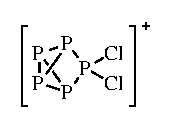
\includegraphics{picture/P5Cl2+.eps}
        \end{minipage}
    }
    \subfigure[\ce{[P5]+}的结构]{
        \begin{minipage}[b]{.2\linewidth}
            \centering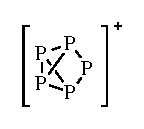
\includegraphics{picture/P5+.eps}
        \end{minipage}
    }
    \subfigure[\ce{[P9]+}的结构]{
        \begin{minipage}[b]{.2\linewidth}
            \centering
\includegraphics{picture/P9+.eps}
        \end{minipage}
    }
    \subfigure[\ce{[P5Ga2Cl6]+}的结构]{
        \begin{minipage}[b]{.3\linewidth}
            \centering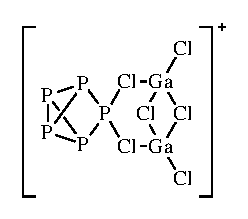
\includegraphics{picture/P5Ga2Cl6+.eps}
        \end{minipage}
    }
    \caption{合成\ce{[P9]+}过程中的各含磷阳离子的结构}
\end{figure}
\ce{[P9+]}中磷的化学位移也耐人寻味.从外到内的磷原子化学位移分别为$-247.49$ ppm,$111.31$ ppm和$60.91$ ppm.
\subsection{磷的氢化物}
\subsubsection{\ce{PH3}}
\begin{substance}[\ce{PH3}]
    磷化氢又名膦,化学式为\ce{PH3},是无色无味(也有说法认为有微弱大蒜气味),可燃且剧毒的气体,熔点为$-132.8\tc$,沸点为$-87.7\tc$.\\
    纯的\ce{PH3}无臭,但工业生产的\ce{PH3}含有\ce{P2H4}等杂质,因此有很臭的腐烂鱼腥味.同样,含有微量\ce{P2H4}的\ce{PH3}在空气中即发生自燃.
\end{substance}
\paragraph{\ce{PH3}的结构}
这是一个值得探讨的问题.\\
\indent 我们已经知道\ce{PH3}的键角为$93.5^\circ$,与\ce{AsH3}和\ce{SbH3}相似,而与\ce{NH3}的$107.8^\circ$相去甚远.国内的教材一般解释为第三周期及以后的元素的p轨道与s轨道能量差距更大,孤对电子倾向占据s轨道,杂化的程度小,因此键角接近$90^\circ$.\\
\indent 一种新的视角是:第二周期的元素实际上才是特殊的\footnote{“来者不善呐”“你才是来者”——姜文, 周润发, 葛优, \textit{让子弹飞}.}.我们知道,所有p轨道中只有2p轨道没有径向节面.而2s轨道有一个径向节面.这就导致了这两个轨道的轨道半径几乎一样大,因此从杂化论的角度而言,这两个轨道能量相近,形成$\text{sp}^n$杂化更加容易.这就是\tbf{量子初轨效应}\footnote{Z.-L. Wang, H.-S. Hu, L. von Szentpály, H. Stoll, S. Fritzsche, P. Pyykkö, W. H. E. Schwarz, J. Li, \textit{Chem. Eur. J.} \tbf{2020}, \textit{26}, 15558-15564, doi.org/10.1002/chem.202003920}.\\
\indent 事实上\footnote{这段内容摘编自\textit{The Nature of the Chemical Bond and the Structure of Molecules and Crystals: An Introduction to Modern Structural Chemistry}.由于Pauling著此书的年代已经较为久远,因此仅供参考.},Pauling最早提出杂化论时就认为\ce{NH3},\ce{H2O}等第二周期元素的氢化物才是特殊的.理论上而言,孤对电子总是应当占据能量最低的s轨道,于是这些物质中的键角总应当接近$90^\circ$.然而,由于第二周期元素较小的共价半径和较大的电负性,如果键角如理论所预期的那样为$90^\circ$,那么这些\ce{H}原子将不可避免地发生明显排斥(无论是体积还是电荷).因此,这些物质的键角明显偏大.\\
\indent 现在,主流的观点认为杂化只是一种数学上的变换,并不对应真实的物理过程.我们应当思考的是“杂化是否能解释\ce{PH3}”而非“\ce{PH3}是否符合杂化理论”.当然,作为一种通俗且一般的理论,我们可以给杂化论打上一些补丁后解释很多东西.不过现在通常采取的更严谨科学的方式是结合这些分子的光电子能谱数据,用分子轨道理论描述其结构\footnote{这可以参考\textit{Orbital Interactions in Chemistry}一书的相关内容.另外,\textit{Modern Physical Organic Chemistry}中也有对分子轨道理论的介绍.}.\\
\indent 一个由此而衍生的问题是\ce{PR3}和\ce{NR3}的构象转换速率.一般的\ce{NR3}不具有手性,因为它能很快速地进行构象反转,而\ce{PR3}则恰好相反.无论是从分子轨道的角度解释(和前面一样,这需要用到Walsh图)还是从杂化论的角度解释(翻转构象需要经过sp$^2$杂化的平面过渡态,这对3s轨道和3p轨道能量差距较大的P元素是很不利的,而N元素就没有这个问题),都可以给出满意的回答.
\paragraph{\ce{PH3}的制备}
可以用若干种方法制备\ce{PH3},现在列举如下:
\begin{enumerate}[label=\tbf{\arabic*.},topsep=0pt,parsep=0pt,itemsep=0pt,partopsep=0pt]
    \item 金属磷化物的水解.例如:
        \begin{center}
            \ce{Ca3P2 + 6H2O -> 2PH3 + 3Ca(OH)2}
        \end{center}
    \item 亚磷酸的热分解:
        \begin{center}
            \ce{4H3PO3 ->T[$200\tc$] PH3 + 3H3PO4}
        \end{center}
    \item \ce{PH4I}的碱解:
        \begin{center}
            \ce{P4 + 2I2 + 8H2O -> 2PH4I + 2HI + 2H3PO4}\\
            \ce{PH4I + KOH -> PH3 + KI + H2O}
        \end{center}
        此法能制得很纯的\ce{PH3}.
    \item 用\ce{H-}还原剂还原\ce{PCl3},例如:
        \begin{center}
            \ce{4PCl3 + 3LiAlH4 -> 4PH3 + 3LiAlCl4}
        \end{center}
    \item 白磷的碱解:
        \begin{center}
            \ce{P4 + 3KOH + 3H2O -> PH3 + 3KH2PO2}
        \end{center}
        这也是工业上制取\ce{PH3}的方法.你可以形象地将其理解为\ce{P4}中的每根\ce{P-P}键都被\ce{OH-}进攻而断裂的结果.
\end{enumerate}
\paragraph{\ce{PH3}的性质与反应}
在水溶液中,\ce{PH3}的酸性和碱性都非常弱:
\begin{center}
    \ce{PH3(aq) + H2O(l) <=> PH^-_2(aq) + H3O+(aq)}\ \ \ $K_\text a=1.6\times10^{-29}$\\
    \ce{PH3(aq) + H2O(l) <=> PH^+_4(aq) + OH-(aq)}\ \ \ $K_\text b=4.0\times10^{-28}$
\end{center}
然而在液氨中,\ce{PH3}溶解形成\ce{NH4PH2}.此外,\ce{PH^+_4}与\ce{Cl-,I-}的盐也是难溶的.\\
\indent 用石墨电极电解\ce{PH3}可以得到\ce{HCN}的类似物\ce{HCP}:
\begin{center}
    \ce{PH3 + C -> HCP + H2}
\end{center}
\indent \ce{PH3}另外一个重要的反应是与酸性甲醛水溶液的反应:
\begin{center}
    \ce{PH3 + 4HCHO + HCl -> [P(CH2OH)4]Cl}
\end{center}
所形成的氯化四羟甲基鏻是一种耐火材料.\ce{NH3}也可以与甲醛反应,但产物并不相同:
\begin{center}
    \ce{4NH3 + 6HCHO + HCl -> [HN4(CH2)6]Cl + 6H2O}
\end{center}
生成六次甲基四胺(乌洛托品)的盐酸盐.
\subsubsection{\ce{P2H4}}
\begin{substance}[\ce{P2H4}]
    四氢化二磷,又称连膦,化学式为\ce{P2H4},是一种无色挥发性的液体.
\end{substance}
连膦可以由对\ce{PH3}放电得到.
\subsection{磷的卤化物}
\subsubsection{\ce{PX3}}
全部四种三卤化物皆为易挥发,易反应的化合物,其分子构型为角锥形.这里把它们的物理性质和结构数据列举如下.
\begin{table}[H]\centering
    \begin{tabular}{ccccc}
        \hline
        物质    &\ce{PF3}   &\ce{PCl3}  &\ce{PBr3}  &\ce{{PI3}} \\\hline
        颜色    &无色       &无色     &无色      &红色 \\
        熔点/$\tc$  &$-151.5$   &$-93.6$    &$-41.5$    &$61.2$ \\
        沸点/$\tc$  &$-101.8$   &$76.1$    &$173.2$     &$>200\tc$分解 \\
        键角    &$96.3^\circ$    &$100^\circ$    &$101^\circ$   &$102^\circ$\\
        键长/pm &$156$  &$204$  &$222$  &$243$\\\hline
    \end{tabular}
\end{table}
\paragraph{对\ce{PX3}键角数据的分析}
我们以\ce{PF3}为例.应当可以发现有如下键角关系:
\begin{center}
    $\ce{NH3}>\ce{NF3}>\ce{PF3}>\ce{PH3}$
\end{center}
这里提供一个简单的规则,即\tbf{本特规则(Bent's rule)}.我们都知道电子在$n$s轨道比在$n$p轨道上更稳定,因此Bent发表了如下规则:
\begin{center}
    原子杂化轨道中,指向电正性取代基的杂化轨道带有较强的s轨道特征.
\end{center}
这是容易理解的.如果中心原子连接了电正性较大的原子,这就意味着这根键的电子更偏向中心原子,也就应当分配更多的s轨道成分.这是除了基团体积效应以外的另一个解释上述结果的理论.
\paragraph{\ce{PX3}的制备}
制备\ce{PF3}的最好方法是将\ce{CaF2},\ce{ZnF2}等氟化剂与\ce{PCl3}反应.其他的三卤化物则利用单质直接卤化而成即可.
\paragraph{\ce{PX3}的性质与反应}
\ce{PF3}作为配体时与\ce{CO}有相似性.正因此,它能与血红蛋白结合,从而体现强烈的毒性.\\
\indent \ce{PF3}仅缓慢水解,而其余\ce{PX3}都迅速地发生水解.反应的通式如下:
\begin{center}
    \ce{PX3 + 3H2O -> H3PO3 + 3HX}
\end{center}

\indent \ce{PCl3}与冷的\ce{N2O4}可以发生不寻常的氧化反应,产物为\ce{P2NOCl5},其结构如下:
\chemfig{P2NOCl5}{1}{\ce{P2NOCl5}的结构}
除此之外,\ce{PCl3}在有机化学中常常作为氯化试剂使用.\\
\indent \ce{PI3}则在有机化学中作为脱氧剂使用.例如,在\ce{NEt3}的协助下,它可以把\ce{RCH=NOH}或\ce{RCH2NO2}高产率地转化为腈.
\subsubsection{\ce{PX5}}
同样地,这里也列举出各\ce{PX5}的物理性质.
\begin{table}[H]\centering
    \begin{tabular}{ccccc}
        \hline
        物质    &\ce{PF5}   &\ce{PCl5}  &\ce{PBr5}  &\ce{{PI5}} \\\hline
        固态组成    &\ce{PF5}   &\ce{[PCl4]+[PCl6]-}    &\ce{[PBr4]+[Br]-} & $-$\\
        颜色    &无色       &灰白色     &浅红黄色      &棕黑色 \\
        熔点/$\tc$  &$-93.7$   &$-167$    &$<100\tc$(分解)    &$41$ \\
        沸点/$\tc$  &$-84.5$   &$>160\tc$(升华)    &$-$     &$-$ \\\hline
    \end{tabular}
\end{table}
\paragraph{对\ce{PX5}结构的分析}
\ce{PF5}分子具有典型的三角双锥结构.轴向的\ce{P-F}键长为$158$ pm,赤道的\ce{P-F}键长为$153$ pm.正如我们建议的那样,中心的磷原子的d轨道几乎不参与成键,因此\ce{PF5}中的\ce{P}实际上采取sp$^2$杂化与赤道的三个\ce{F}原子连接,轴向的p轨道与两个\ce{F}原子形成三中心四电子键.这导致了轴向键的键级更接近$0.5$.你可以简单地认为轴向的键的共价性较弱,而电荷作用弥补了这一点.\\
\indent 这一成键性质又可以导出另一个有趣的结果.在所有\ce{PF_{n}Cl_{5-n}}分子中,\ce{F}总是优先占据轴向的位置.这正是符合本特规则的,因为高电负性的F原子所成的键理当优先占据p轨道成分更高的轴向位置.
\paragraph{\ce{PX5}的性质与反应}
\ce{PF5}是优良的\ce{F-}离子受体.\ce{[PF6]-}由于其优异的稳定性,经常作为有机盐类的反号离子参与反应.\\
\indent 在气相中,\ce{PCl5}存在如下平衡:
\begin{center}
    \ce{PCl5 <=> PCl3 + Cl2}
\end{center}
工业上利用\ce{Cl2}对\ce{PCl3}氯化以制取\ce{PCl5}.它在水中猛烈地水解为\ce{H3PO4}和\ce{HCl},但倘若使用等摩尔的水则反应减缓,同时生成\ce{POCl3}:
\begin{center}
    \ce{PCl5 + 4H2O -> H3PO4 + 5HCl}\\
    \ce{PCl5 + H2O -> POCl3 + 2HCl}
\end{center}
\ce{PCl5}也是优良的强氯化试剂.\\
\indent \ce{PBr5}加热后即分解为\ce{PBr3}与\ce{Br2}.骤冷此混合气体可以得到\ce{PBr3}与\ce{PBr7}(即\ce{[PBr4]+[Br3]-})的混合物.
\subsubsection{\ce{P2X4}}
\ce{P2X4}并不常见,其性质也与\ce{PX3}和\ce{P2H4}有一定相似之处.\ce{P2F4}可以由偶联法制得:
\begin{center}
    \ce{2PF2I + 2Hg -> P2F4 + Hg2I2}
\end{center}
\ce{P2Cl4}则可以通过对\ce{PCl3}放电得到.
\subsection{磷的氧化物和硫化物}
\subsubsection{各类磷的氧化物和硫化物的结构}
这里给出各类磷的氧化物和硫化物的结构.
\begin{figure}[H]
    \centering
    \subfigure[\ce{P4O6}]{
        \begin{minipage}[b]{.3\linewidth}
            \centering
\includegraphics{picture/P4O6.eps}
        \end{minipage}
    }
    \subfigure[\ce{P4O7}]{
        \begin{minipage}[b]{.3\linewidth}
            \centering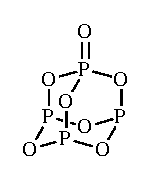
\includegraphics{picture/P4O7.eps}
        \end{minipage}
    }
    \subfigure[\ce{P4O8}]{
        \begin{minipage}[b]{.3\linewidth}
            \centering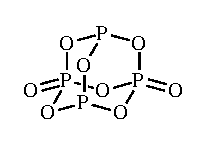
\includegraphics{picture/P4O8.eps}
        \end{minipage}
    }
    \subfigure[\ce{P4O9}]{
        \begin{minipage}[b]{.3\linewidth}
            \centering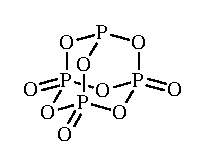
\includegraphics{picture/P4O9.eps}
        \end{minipage}
    }
    \subfigure[\ce{P4O10}]{
        \begin{minipage}[b]{.3\linewidth}
            \centering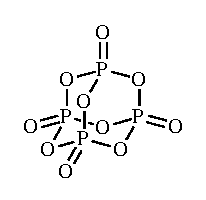
\includegraphics{picture/P4O10.eps}
        \end{minipage}
    }\caption{各类磷的氧化物的结构}
\end{figure}
\begin{figure}[H]
    \centering
    \subfigure[\ce{P4S3}]{
        \begin{minipage}[b]{.23\linewidth}
            \centering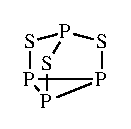
\includegraphics{picture/P4S3.eps}
        \end{minipage}
    }
    \subfigure[$\alpha$-\ce{P4S4}]{
        \begin{minipage}[b]{.23\linewidth}
            \centering
\includegraphics{picture/alpha-P4S4.eps}
        \end{minipage}
    }
    \subfigure[$\beta$-\ce{P4S4}]{
        \begin{minipage}[b]{.23\linewidth}
            \centering
\includegraphics{picture/beta-P4S4.eps}
        \end{minipage}
    }
    \subfigure[\ce{P4S5}]{
        \begin{minipage}[b]{.23\linewidth}
            \centering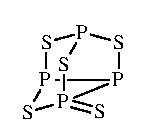
\includegraphics{picture/P4S5.eps}
        \end{minipage}
    }
    \subfigure[\ce{P4S7}]{
        \begin{minipage}[b]{.23\linewidth}
            \centering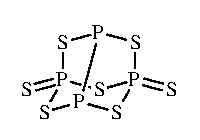
\includegraphics{picture/P4S7.eps}
        \end{minipage}
    }
    \subfigure[\ce{P4S9}]{
        \begin{minipage}[b]{.23\linewidth}
            \centering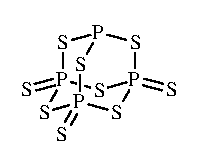
\includegraphics{picture/P4S9.eps}
        \end{minipage}
    }
     \subfigure[\ce{P4S10}]{
        \begin{minipage}[b]{.23\linewidth}
            \centering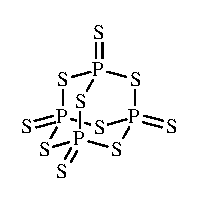
\includegraphics{picture/P4S10.eps}
        \end{minipage}
    }\caption{各类磷的硫化物的结构}
\end{figure}
\subsubsection{磷的氧化物}
\begin{substance}[\ce{P4O6}]
    三氧化二磷,化学式为\ce{P4O6},是一种白色蜡状有大蒜气味的极毒晶体,熔点为$23.8\tc$,沸点为$173\tc$.
\end{substance}
\begin{substance}[\ce{P4O10}]
    五氧化二磷,化学式为\ce{P4O10},是一种白色粉末,有强烈的吸水性,在$360\tc$升华.
\end{substance}
\paragraph{\ce{P4O10}和\ce{P4O6}的制备,性质和用途}
\ce{P4O6}可以由白磷在限量空气中燃烧得到,而\ce{P4O10}则可以由白磷在足量空气中燃烧得到.\\
\indent \ce{P4O6}和\ce{P4O10}均可以水解,但后者容易得多.
\begin{center}
    \ce{P4O6 + 6H2O -> 4H3PO3}
\end{center}
而\ce{P4O10}与水发生剧烈的反应,因此可以作为脱水剂使用.它使\ce{RCONH2}脱水为\ce{RCN},使\ce{HNO3}脱水为\ce{N2O5},等等.脱水时的产物一般为偏磷酸\ce{HPO3}.\\
\indent \ce{P4O10}的最大用途是生产正磷酸和多磷酸.此外,它还可以用于生产磷酸酯,例如:
\begin{center}
    \ce{P4O10 + 6Et2O -> 4PO(OEt)3}
\end{center}

\indent \ce{P4O6}也可以作为一种优良的配体,例如它可以逐步取代\ce{Ni(CO)4}中的\ce{CO}形成一系列配合物.
\paragraph{磷的其它氧化物} 磷的低氧化物\ce{OP}可以由下面的反应制得:
\begin{center}
    \ce{2POBr3 + 3Mg -> 3MgBr2 + 2OP}
\end{center}

\indent 低压下将\ce{P4O10}与\ce{O2}混合后放电可以得到\ce{P2O6}.其结构可能是\ce{P4O10}中的氧桥被替换为过氧桥.\\
\indent \ce{P4O6}在低温下与\ce{O3}反应可以得到\ce{P4O18},其结构如下:
\chemfig{P4O18}{1}{\ce{P4O18}的立体结构}
这一物质不稳定,容易释放\ce{O2}而形成\ce{P4O10}.
\subsubsection{磷的硫化物}
\paragraph{磷的硫化物的制备与性质}
\ce{P4S3}是磷最稳定的硫化物,可以由红磷与计量的硫加热得到.\ce{P4S7}是稳定性仅次于\ce{P4S3}的磷的硫化物,其中令人费解的保留了一根\ce{P-P}键同时有两个端基\ce{S}原子.\\
\indent \ce{P4S10}是磷在工业上最重要的硫化物,可利用液态白磷与稍过量的硫在高于$300\tc$时直接反应生成.它也可由工业制硫单质的副产品磷铁制得:
\begin{center}
    \ce{4Fe2P + 18FeS2 -> P4S10 + 26FeS}
\end{center}
\ce{P4S10}的结构与\ce{P4O10}基本一致.它主要按照以下方式水解:
\begin{center}
    \ce{P4S10 + 16H2O -> 4H3PO4 + 10H2S}
\end{center}
\paragraph{工业上的磷硫化物}
有两种重要的化合物\ce{P4S3}和\ce{P4S10}.\\
\indent \ce{P4S3}主要用于生产火柴头.这种火柴在任意表面摩擦均可起火,因为它的反应物\ce{KClO3}和\ce{P4S3}被混合于火柴头上.目前使用的安全火柴大部分都将\ce{KClO3}填充于火柴头上,而将红磷作为涂料附在火柴盒侧面,两者摩擦时反应而起火.\\
\indent \ce{P4S10}是大量有机\ce{P}-\ce{S}化合物的主要来源,可以用于生产农药.此外,它与醇或酚反应生成的二硫代磷酸二酯可以用于润滑油的添加剂:
\begin{center}
    \ce{P4S10 + 8ROH -> 4(RO)2P(S)SH + 2H2S}
\end{center}
\subsection{磷的卤氧化物}
\subsubsection{\ce{POCl3}}
\begin{substance}[\ce{POCl3}]
    三氯氧磷,化学式为\ce{POCl3},是无色澄清液体,潮湿空气中发烟.\ce{POCl3}的熔点为$1.25\tc$,沸点为$105.8\tc$.
\end{substance}
\paragraph{\ce{POCl3}的制备}
室温下\ce{PCl3}很容易与\ce{O2}反应生成\ce{POCl3}:
\begin{center}
    \ce{2PCl3 + O2 -> 2POCl3}
\end{center}
又或者将\ce{P4O10}溶于\ce{PCl3}后进行氯化,生成的\ce{PCl5}又与\ce{P4O10}反应而生成\ce{POCl3}:
\begin{center}
    \ce{P4O10 + 6PCl5 -> 10POCl3}
\end{center}
\paragraph{\ce{POCl3}的反应}
也许\ce{POCl3}最著名的反应是Vilsmeier-Haack反应.这一反应以\ce{DMF}和\ce{POCl3}作为甲酰化试剂.\\
\indent 此外,\ce{POCl3}也可以作为一种典型的非水溶剂和配体.它自身能发生电离:
\begin{center}
    \ce{$(n+1)$ POCl3 <=> POCl2^+ + [Cl(POCl3)_n]^-}
\end{center}
又如不同的物质在\ce{POCl3}中发生的溶剂解反应:
\begin{center}
    \ce{4AlCl3 + 6POCl3 -> [Al[POCl3]6][AlCl4]3}\\
    \ce{4AlI3 + 18POCl3 -> [Al[POCl3]6][AlCl4]3 + 12POICl2}\\
    \ce{SbCl5 + POCl3 -> [POCl2][SbCl6]}
\end{center}
诸如此类等等.
\subsubsection{其它卤氧化物}
把\ce{Cl2}通到沸腾的用\ce{CCl4}稀释的\ce{P4O10}和\ce{PCl3}悬浮液中,可方便地制得焦磷酰基氯化物\ce{P2O3Cl4}:
\begin{center}
    \ce{P4O10 + 4PCl3 + 4Cl2 -> 2P2O3Cl4 + 4POCl3}
\end{center}
其结构如下:
\chemfig{P2O3Cl4}{1}{\ce{P2O3Cl4}分子的结构}
\subsection{磷的含氧酸}
\subsubsection{次磷酸及其盐}
\paragraph{次磷酸及其盐的制备}
次磷酸盐可以通过\ce{P4}与热的强碱水溶液反应制得:
\begin{center}
    \ce{P4 + 4OH- + 4H2O ->T[$\Delta$] 4H2PO2- + 2H2} 
\end{center}
此反应的副产物主要是\ce{HPO3^2-}和\ce{PH3}.前者可以通过形成钙盐沉淀的方式去除,后者则会自动地逸出体系:
\begin{center}
    \ce{P4 + 2Ca(OH)2 + 2H2O -> 2CaHPO3 v + 2PH3}
\end{center}
酸化次磷酸盐的水溶液就可以得到\ce{H3PO2}的水溶液.用\ce{Et2O}萃取即得纯\ce{H3PO2},它是白色晶体,熔点为$26.5\tc$,同时也是一元弱酸,$\text pK_\text a=1.1$.
\paragraph{次磷酸盐的应用}
次磷酸盐(尤其是次磷酸钠)常用于工业还原剂.特别地,它被用于化学镀镍:
\begin{center}
    \ce{Ni^2+ + H2PO2- + OH- -> Ni + HPO3^2- + H2O}
\end{center}
此外,次磷酸盐还可以将芳香重氮盐\ce{Ar-N2+}还原为芳烃\ce{Ar-H}.这在利用定位效应合成多取代芳环时可能用到.
\subsubsection{亚磷酸及其盐}
\paragraph{亚磷酸的制备}
前面已经说过,亚磷酸可以由\ce{PCl3}水解得到:
\begin{center}
    \ce{PCl3 + 3H2O -> H3PO3 + 3HCl}
\end{center}
\paragraph{亚磷酸酯的制备}
一般而言,\ce{PCl3}与\ce{ROH}的反应即可制得亚磷酸酯,但会随着条件不同产生两种异构体:
\begin{center}
    \ce{PCl3 + 3ROH -> HPO(OR)2 + RCl + 2HCl}\\
    \ce{PCl3 + 3ROH + 3Et3N -> P(OR)3 + 4Et3NHCl}
\end{center}
如果采用酚类反应,那么无需加碱即可生成\ce{P(OAr)3}.然而,\ce{P(OMe)3}会自动地发生异构化:
\begin{center}
    \ce{P(OMe)3 -> MePO(OMe)2}
\end{center}
总之这些反应是令人费解而神奇的.
\subsubsection{磷酸及其盐}
\paragraph{无水磷酸的性质}
无水磷酸\ce{H3PO4}几乎总是和焦磷酸和各种多磷酸处在平衡之中.典型的平衡如下:
\begin{center}
    \ce{2H3PO4 <=> H2O + H4P2O7}\\
    \ce{2H3PO4 <=> H4PO4+ + H2PO4-}\\
    \ce{H2O + H3PO4 <=> H3O+ + H2PO4-}\\
    \ce{H4P2O7 + H3PO4 <=> H4PO4+ + H3P2O7-}\\
    \ce{H3P2O7- + H3PO4 <=> H4PO4+ + H2P2O7^2-}
\end{center}
错综复杂的氢键网络使得无水磷酸有极高的粘度.由于粘度过高,正常的离子迁移很难发生,但无水磷酸仍具有很高的电导率.与\ce{H2O}类似,氢键网络使得\ce{H+}可以迅速地在分子间发生传递.
\paragraph{磷酸水溶液的性质}
在水溶液中,\ce{H3PO4}表现为三元中强酸:
\begin{center}
    \ce{H3PO4 + H2O <=> H3O+ + H2PO4-}\ \ \ $K_{\text a1}=7.11\times10^{-3}$\\
    \ce{H2PO4- + H2O <=> H3O+ + HPO4^2-}\ \ \ $K_{\text a1}=6.31\times10^{-8}$\\
    \ce{HPO4^2- + H2O <=> H3O+ + PO4^3-}\ \ \ $K_{\text a1}=4.22\times10^{-13}$
\end{center}
分析化学上常用的磷酸缓冲溶液就是由等浓度的\ce{Na2HPO4}和\ce{KH2PO4}混合而成.
\paragraph{磷酸的制备与用途}
磷酸是化工行业重要的酸.制备浓磷酸主要采用\ce{P4}在\ce{O2}与\ce{H2O}的混合物中燃烧:
\begin{center}
    \ce{P4 + 5O2 + 6H2O -> 4H3PO4}
\end{center}
以前也采用硫酸与氟磷灰石反应的方法:
\begin{center}
    \ce{Ca5(PO4)3F + 5H2SO4 + 10H2O -> 3H3PO4 + 5CaSO4.2H2O + HF}
\end{center}
磷酸在工业上的用途非常广泛.此外,磷酸根离子在分析化学中也常用作掩蔽\ce{Fe^3+}的试剂.此外,磷酸也可以作为食品添加剂而被使用,碳酸饮料中就主要是磷酸体现酸性.
\paragraph{磷酸盐的用途}
\ce{Na3PO4}在水溶液中呈现明显的碱性,因而是洗涤粉,洗漆剂和油脂皂化剂的重要成分.\\
\indent\ce{Na2HPO4}亦有广泛的用途,主要用于水的软化和各类食品的添加剂.\\
\indent 过磷酸钙实际上并非过氧磷酸的钙盐,甚至不是纯净物,而是稀硫酸与磷矿石反应的固体产物.例如:
\begin{center}
    \ce{2Ca5(PO4)3F + 7H2SO4 + H2O -> 7CaSO4 + 3Ca(H2PO4)2.H2O + 2HF}
\end{center}
过磷酸钙主要在农业上用作磷肥,其中的\ce{CaSO4}并无用处.因此,也可以用\ce{H3PO4}代替\ce{H2SO4}得到三过磷酸钙:
\begin{center}
    \ce{Ca5(PO4)3F + 7H3PO4 + H2O -> 5Ca(H2PO4)2.H2O + HF}
\end{center}
三过磷酸钙的有效\ce{P2O5}含量几乎是过磷酸钙的三倍,因而得名.\\
\indent 人体的骨骼的主要成分是羟基磷灰石\ce{Ca5(PO4)3(OH)}.
\paragraph{焦磷酸盐}
焦磷酸盐通常可以通过以下方法制备:
\begin{enumerate}[label=\tbf{\arabic*.},topsep=0pt,parsep=0pt,itemsep=0pt,partopsep=0pt]
    \item 磷酸一氢盐或磷酸二氢盐的热缩合反应.
        \begin{center}
            \ce{2MH2PO4 ->T[$\Delta$] M2H2P2O7 + H2O}\ \ \ \ \ \ce{2M2HPO4 ->T[$\Delta$] M4P2O7 + H2O}
        \end{center}
    \item \ce{H3PO4}与氧化物反应.
        \begin{center}
            \ce{PbO2 + 2H3PO4 -> PbP2O7 v + 3H2O}
        \end{center}
    \item 各种磷酸盐的热分解.
        \begin{center}
            \ce{8Cr(PO3)3 ->T[$\Delta$] 2Cr4(P2O7)3 + 3P4O10}\ \ \ \ \ \ce{2Hg3(PO4)2 ->T[$\Delta$] 2Hg2P2O7 + 2Hg + O2}
        \end{center}
\end{enumerate}
\indent \ce{Na4P2O7}和\ce{Na2H2P2O7}都可以作为食品添加剂.\ce{Ca2P2O7}则可以作为牙膏磨料,涂料填料等.
\paragraph{三聚磷酸盐}
最重要的三聚磷酸盐即三聚磷酸钠.它可以由下面的方法合成:
\begin{center}
    \ce{2Na2HPO4 + NaH2PO4 -> Na5P3O10 + 2H2O}
\end{center}
\ce{Na5P3O10}常用于制造合成洗涤剂.\\
\indent 腺苷三磷酸(ATP)中也含有三聚磷酸结构.它的水解会释放大量能量,因此作为生物体内最直接的能量来源.
\subsubsection{连二磷酸及其盐}
连二磷酸通常是在室温下用\ce{NaClO2}溶液控制地氧化红磷而制得:
\begin{center}
    \ce{2P + 2NaClO2 + 2H2O -> Na2H2P2O6 + 2HCl}
\end{center}
连二磷酸中含有一根\ce{P-P}键,其结构如下.异连二磷酸则可以由化学计量的\ce{H3PO4}和\ce{H2O}使\ce{PCl3}脱水得到,%
实际上可以描述为亚磷酸和磷酸的混合酸酐,其结构在下面一并示出.
\begin{figure}[H]
    \centering
    \subfigure[连二磷酸]{
        \begin{minipage}[b]{.45\linewidth}
            \centering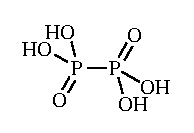
\includegraphics{picture/H4P2O6-1.eps}
        \end{minipage}
    }
    \subfigure[异连二磷酸]{
        \begin{minipage}[b]{.45\linewidth}
            \centering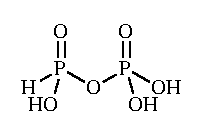
\includegraphics{picture/H4P2O6-2.eps}
        \end{minipage}
    }\caption{两种连二磷酸的结构}
\end{figure}
\subsection{磷氮化合物}
鉴于磷氮化合物复杂的种类和反应,这部分内容请自行查阅相关资料.在这里仅给出一些经典的反应与结构.\\
\indent \ce{PCl5}在\ce{NH3(l)}中发生氨解:
\begin{center}
    \ce{2PCl5 + 16NH3 -> [(H2N)3PNP(NH2)3]Cl + 9NH4Cl}
\end{center}
产物和焦磷酸的结构比较相似.\\
\indent \ce{PCl5}和\ce{NH4Cl}在合适的情况下发生热解可得\ce{N7P6Cl9}.这是一个并环化合物,其结构如下:
\chemfig{N7P6Cl9}{1}{\ce{N7P6Cl9}的结构}
\end{document}